% ============================================================
\section{Zakořeněné a binární stromy}
% ============================================================

Od tohoto momentu se postupně začneme bavit o datovách strukturách. Jako první si zavedeme pomocné definice zakořenění a binárního stromu. Pomocí nich budeme poté definovat další datové struktury. Např. binární vyhledávací strom nebo minimovou haldu. \bigskip

\begin{definition}[Zakořeněný strom]
\leavevmode
\begin{itemize}
    \item \textbf{Zakořeněný strom} je strom $T$, ve kterém je jeden vrchol $r \in V(T)$ označen jako \textbf{kořen}. 
    \item Leží-li vrchol $u$ na (jediné) cestě z vrcholu $v$ do kořene $r$, pak $u$ nazveme \textbf{předkem} vrcholu $v$ a $v$ nazveme \textbf{potomkem} vrcholu $u$.
    \item Pokud navíc $\{u, v\} \in E(T)$ tvoří hranu, říkáme, že $u$ je \textbf{otec} (rodič) vrcholu $v$ a $v$ je \textbf{syn} (dítě) vrcholu $u$.
    \item Vrcholy rozřazujeme podle vzdálenosti od kořene do jednotlivých \textbf{hladin}: v 0.\ hladině leží samotný kořen $r$, v 1.\ hladině leží jeho synové atd.
    \item \textbf{Hloubka zakořeněného stromu} $T$ je celkový počet jeho hladin.
\end{itemize}
\end{definition} \bigskip

\begin{definition}[Binární strom]
Strom nazveme \textbf{binární}, pokud:
\begin{enumerate}
    \item je zakořeněný,
    \item každý vrchol má nejvýše dva syny,
    \item u synů rozlišujeme, který je \textbf{levý} a který \textbf{pravý}.
\end{enumerate}
\end{definition} \bigskip

\begin{center}
    \begin{figure}[H]
\centering
\begin{tikzpicture}[
  vnode/.style={circle, draw, minimum size=7mm, inner sep=0pt, fill=blue!10},
  thick, level distance=12mm,
  level 1/.style={sibling distance=30mm},
  level 2/.style={sibling distance=16mm}
]
  \node[vnode, fill=red!20] (r) {$r$}
    child { node[vnode] (a) {$a$}
      child { node[vnode] (c) {$c$} }
      child { node[vnode] (d) {$d$} }
    }
    child { node[vnode] (b) {$b$}
      child { node[vnode] (e) {$e$} }
      child[missing]
    };
    
  \node[right=20mm of r, gray] {0. hladina (kořen $r$)};
  \node[right=35mm of a, gray] {1. hladina (synové $a, b$)};
  \node[right=43mm of c, gray] {2. hladina (synové $c, d, e$)};
\end{tikzpicture}
\caption{Ukázka zakořeněného binárního stromu s hloubkou 3.}
\end{figure}
\end{center}

\newpage

% ============================================================
\section{Binární minimová halda}
% ============================================================

První datovou strukturou je binární minimová halda. Je velmi důležitá, pomocí ní dokážeme efektivně získávat minima z množiny prvků. Alternativně u maximové maxima, nebo mediánové medián apod. Pomocí ní je implementována např. prioritní fronta v c++. Dále je možné pomocí ní řadit díky algoritmu HeapSort. \medskip

\noindent Halda drží pevnou strukturu, vždy ji naplňujeme zhora-dolů a zleva-doprava. Zároveň u ní platí, že kořen je nejmenším z prvků. A pro všechny prvky platí, že jejich otec je menší než oni sami. Mezi sousedy žádné takové pravidlo neplatí. \bigskip

\begin{definition}[Binární minimová halda]
\textbf{Binární minimová halda} (zkráceně jen \textbf{halda}) je datová struktura ve tvaru binárního stromu, v jehož každém vrcholu $x$ je uložen jeden porovnatelný klíč $k(x)$, přičemž splňuje dvě základní podmínky:
\begin{enumerate}
    \item \textbf{Tvar haldy:} Strom má všechny hladiny kromě poslední zcela plně obsazené. Poslední hladina je zaplněna souvisle od levého okraje směrem k pravému.
    \item \textbf{Haldové uspořádání:} Pro každý vrchol $v$ a pro libovolného jeho syna $s$ platí:
    $$k(v) \le k(s)$$
\end{enumerate}
\end{definition} \bigskip

\begin{remark}[Pozorování]
Z podmínek haldového uspořádání plyne, že na libovolné cestě vedoucí z jakéhokoli vrcholu nahoru do kořene tvoří klíče \textbf{nerostoucí} posloupnost. V samotném kořeni haldy se tedy vždy nachází \textbf{globální minimum} ze všech uložených prvků.
\end{remark} \bigskip

\begin{center}
    \begin{figure}[H]
\centering
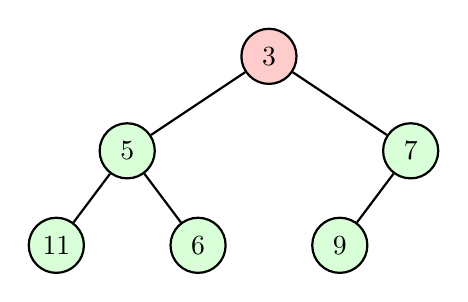
\begin{tikzpicture}[
  vnode/.style={circle, draw, minimum size=7mm, inner sep=0pt, fill=green!15},
  thick, level distance=12mm,
  level 1/.style={sibling distance=36mm},
  level 2/.style={sibling distance=18mm},
  level 3/.style={sibling distance=10mm}
]
  \node[vnode, fill=red!20] (n3) {$3$}
    child { node[vnode] (n5) {$5$}
      child { node[vnode] (n11) {$11$} }
      child { node[vnode] (n6) {$6$} }
    }
    child { node[vnode] (n7) {$7$}
      child { node[vnode] (n9) {$9$} }
      child[missing]
    };
\end{tikzpicture}
\caption{Případ binární minimové haldy. Všimněte si, že každá rodičovská hodnota je menší nebo rovna svým synům a poslední hladina je zaplněna zleva.}
\end{figure}
\end{center}

\bigskip

\begin{remark}[Atributy haldy]
Pro formální praci s haldou $H$ udržujeme následující atributy:
\begin{itemize}
    \item $H.root$ -- ukazatel na aktuální kořen haldy,
    \item $H.n$ -- aktuální počet prvků uložených v haldě,
    \item $H.last$ -- ukazatel na aktuálně poslední list (nejpravější prvek v nejspodnější hladině).
\end{itemize}
\end{remark} \bigskip

% ------------------------------------------------------------
\subsection{Strukturální vlastnosti haldy}

\begin{lemma}[Počet hladin haldy]
Binární halda obsahující $n$ prvků má právě $\floor{\log_2 n} + 1$ hladin.
\end{lemma} \bigskip

\begin{proof}
\leavevmode
Uvažujme plně obsazený binární strom o $h \ge 1$ hladinách (od hladiny $0$ do $h - 1$). Počet prvků je součtem geometrické řady:
$$n = 2^0 + 2^1 + 2^2 + \dots + 2^{h-1} = 2^h - 1$$
Kvůli tvaru haldy přibude do haldy nová $h$-tá hladina, když počet prvků $n$ vzroste z $2^h - 1$ na $2^h$. Všimněme si, že hodnota výrazu $\floor{\log_2 (n)}$ se zvětší o 1 přesně při tomto přechodu $n = 2^h$.
Pro $n = 2^h - 1$ dostáváme:
$$h = (h - 1) + 1 = \floor{\log_2(2^h - 1)} + 1 = \floor{\log_2 (n)} + 1$$
\end{proof} \medskip

\noindent Poslední rovnice funguje takto: Víme, že halda drží strukturu binárního stromu, pro $n = 2^h - 1$ (tedy úplný binární strom) má přesně $\log_2 (n)$ hladin. Spodní hodnota tam je pro počet prvků mezi $2^{h-1}$ a $2^h - 1$. A z toho plyne druhá rovnost.\bigskip

\begin{lemma}[Počet listů a vnitřních vrcholů haldy]
Binární halda s $n \ge 3$ prvky má právě $\floor{n/2}$ vnitřních vrcholů a $\ceil{n/2}$ listů.
\end{lemma} \bigskip

\noindent Tento důkaz je velmi mechanický a dokážeme ho pomocí indukce. Stačí nám zohlednit případ kdy má halda sudou a lichou velikost kvůli zaokrouhlování.

\begin{proof}
Důkaz provedeme matematickou indukcí podle počtu vrcholů $n$.
\begin{itemize}
    \item \textbf{Základní krok ($n = 3$):} Halda má kořen (1 vnitřní vrchol) a 2 syny (2 listy). Platí $\floor{3/2} = 1$ a $\ceil{3/2} = 2$. Tvrzení platí.
    \item \textbf{Indukční krok:} Předpokládejme, že tvrzení platí pro všechna $n' < n$. Rozlišme dva případy podle parity $n$:
    \begin{enumerate}
        \item \textbf{$n > 3$ je liché:} Poslední list $l$ je pravým synem svého otce. Jeho odebráním vznikne halda o sudé velikosti $n$ - 1. Z indukčního předpokladu má tato menší halda $\ceil{(n-1)/2}$ listů a $\floor{(n-1)/2}$ vnitřních vrcholů. Navrácením listu $l$ se počet vnitřních vrcholů nezmění (jeho otec už byl vnitřním vrcholem jako otec levého syna), tedy počet vnitřních vrcholů je $\floor{(n-1)/2} = \floor{n/2}$. Počet listů vzroste o 1:
        $$\ceil{\frac{n-1}{2}} + 1 = \frac{n-1}{2} + 1 = \frac{n+1}{2} = \ceil{\frac{n}{2}}$$
        \item \textbf{$n \ge 4$ je sudé:} Poslední list $l$ je jediným levým synem svého otce. Jeho odebráním vznikne halda liché velikosti $n - 1$. Navrácením listu $l$ se jeho otec stane novým vnitřním vrcholem (přibude 1 vnitřní vrchol) a počet listů se nezmění (otec přestal být listem, ale přibyl list $l$). Tedy počet vnitřních vrcholů je:
        $$\floor{\frac{n-1}{2}} + 1 = \frac{n-2}{2} + 1 = \frac{n}{2} = \floor{\frac{n}{2}}$$
        a počet listů je $\ceil{(n-1)/2} = n/2 = \ceil{n/2}$.
    \end{enumerate}
\end{itemize}
\end{proof}

\newpage

% ============================================================
\section{Základní operace nad haldou}
% ============================================================

Halda má tři základní operace, které provádí efektivně. A to HeapInsert, HeapFindMin a HeapExtractMin. Z názvu plyne co dělají a nyní si ukážeme jejich implementaci. \bigskip

\subsection{Vyhledání minima (HeapFindMin)}
Nalezení minimálního prvku je triviální díky vlastnosti haldového uspořádání. Globální minimum se nachází vždy v kořeni a na ten si držíme ukazatel. Stihneme to určitě za $\bigO{1}$. \bigskip

\funkce{HeapFindMin}{halda $H$}
\begin{pseudocode}
\item return $H.root$
\end{pseudocode} \medskip

\subsection{Vložení prvku (HeapInsert)}
Při vkládání nového klíče $x$ vytvoříme nový vrchol $v$ a rovnou ho vložíme jako nejpravějšího syna na poslední hladině. Jenže jsme tím mohli rozbít haldové uspořádání, tedy že otec $o$ bude najednou větší než $k$, $k(o)$ > $x$. V tomto případě musíme vrcholy $v$ a $o$ prohodit (druhého syna nerozbijeme, jelikož je větší než otec a toho vyměníme za menší prvek). Tento problém se může opakovat až cestou do kořene, a tak prohazujeme dokud je to potřeba. V nejextrémějším případě se z vrcholu $v$ stane kořen, tedy globální minimum. Této operaci opravy říkáme BubbleUp. Díky logaritmické hloubce haldy stihneme celý HeapInsert za $\bigO{\log(n)}$.\bigskip

\funkce{HeapInsert}{halda $H$, klíč $k$}
\begin{pseudocode}
\item $H.n := H.n + 1$
\item Vlož na první volnou pozici v poslední hladině nový vrchol $p$ s klíčem $k$
\item \textcolor{blue}{BubbleUp}($H, p$)
\end{pseudocode} \bigskip

\funkce{BubbleUp}{halda $H$, uzel $p$}
\begin{pseudocode}
\item Dokud $p \neq H.root$:
\item \tab $o := \text{otec}(p)$
\item \tab Pokud $k(o) \le k(p)$: return \hfill {\color{gray}{//Halda je již opravená}}
\item \tab Prohoď $k(o)$ a $k(p)$
\item \tab $p := o$
\end{pseudocode} \bigskip

\begin{remark}
    Zde prohazujeme pouze samotné klíče, jelikož jsme si haldu definovali pouze s klíči. Pokud ale na klíči máte navázanou nějakou hodnotu. Je potřeba prohodit celé vrcholy, aby jste neporušili vazbu (klič, data).
\end{remark} \bigskip

\begin{lemma}[Korektnost a složitost HeapInsert]
Volání operace $\text{HeapInsert}(H, k)$ nad minimovou haldou $H$ vytvoří korektní minimovou haldu v čase $\bigO{\log (n)}$.
\end{lemma}

\begin{proof}
Pokud H je prázdná, pak je výsledkem jednoprvková halda – hotovo. V opačném případě označme K výsledek volání HeapInsert$(H, k)$. K jistě splňuje tvar haldy. Zbývá ověřit, že splňuje podmínku haldového uspořádání. Po přidání hodnoty $k$ do nového listu $l$ může být porušená podmínka mezi $l$ a jeho otcem $o$, tedy $k(l) < k(o)$. Zároveň nemůžeme porušit podmínku s druhým synem $r$ vrcholu $o$, jelikož pro něj platí $k(r) \geq k(o) > k(l)$. Toto řeší procedura BubbleUp, která prohozením posune problém o hladinu blíže ke kořeni a zastaví se nejpozději právě v něm. Již víme, že halda má $\floor{\log_2(n)} + 1$ hladin. Na každé hladině provedeme konstantní množství operací a proto opravíme haldu za $\bigO{\log(n)}$.
\end{proof}

\newpage

\subsection{Odebrání minima (HeapExtractMin)}
Kořen nemůžeme odstranit přímo, jelikož by jsme těžko hledali další minimum (museli by jsme projít celou haldu, tedy by nám operace trvala lineární čas). Proto se využívá trik. Prohodíme klíč v kořeni s klíčem $H.last$. Poslední list poté jednoduše odstraníme. Jenže náš nový klíč v kořeni nyní pravděpodobně porušuje haldové uspořádání. A tak ho postupně zabubláme dolů pomocí prohození vždy s menším z klíčů synů. Každé prohození zabere konstantní množství operací a hladin je v haldě logaritmicky, tedy to stihneme za $\bigO{\log(n)}$.\bigskip

\funkce{HeapExtractMin}{halda $H$}
\begin{pseudocode}
\item $r := H.root,\ x := k(r),\ l := H.last$
\item Prohoď klíče $k(r)$ a $k(l)$
\item $H.n := H.n - 1$ \hfill \textcolor{gray}{// Odstraní poslední list $l$}
\item \textcolor{blue}{BubbleDown}($r$)
\item Vrať $x$
\end{pseudocode} \bigskip

\funkce{BubbleDown}{uzel $v$}
\begin{pseudocode}
\item Dokud má $v$ nějaké syny:
\item \tab $s := \text{syn vrcholu } v \text{ s nejmenším klíčem}$
\item \tab Pokud $k(v) \le k(s)$: return
\item \tab Prohoď klíče $k(v)$ a $k(s)$
\item \tab $v := s$
\end{pseudocode} \bigskip

\begin{lemma}[Korektnost a složitost HeapExtractMin]
Volání $\text{HeapExtractMin}(H)$ odstraní a vrátí minimální prvek z haldy a zachová strukturu minimové haldy v čase $\bigO{\log(n)}$.
\end{lemma} \bigskip

\begin{proof}
Prohozením klíčů a odstraněním posledního listu $l$ jistě zachováme tvar haldy. Náš nový klíč v kořeni může ale porušovat haldové uspořádání. Toto opravuje procedura BubbleDown, která porovná vrchol $v$ s jeho menším synem $s$. Pokud $k(v) \leq k(s)$ končíme. V opačném případě je prohodí. Zároveň zůstane v pořádku druhý syn $d$ vrcholu $v$ jelikož $k(d) \geq k(s)$, což vyžaduje haldové uspořádání. Tímto jsme problém posunuli o hladinu níže. V nejhorším případě takto pokračujeme až do listu, kde algoritmus definitivně skončí. Díky tomu, že halda má logaritmicky hladin a každou operaci provedeme v konstatním čase. Zvládneme celý HeapExtractMin za $\bigO{\log(n)}$.
\end{proof}

\newpage

% ============================================================
\section{Reprezentace haldy v poli}
% ============================================================

Díky pevnému tvaru haldy máme výbornou výhodu a tou je reprezentace v poli. Tato vlastnost se nám následně bude hodit pro řazení pole pomocí algoritmu HeapSort. \bigskip

\noindent Haldu postupně indexujeme zhora-dolů a zleva-doprava. Kořen začíná na indexu 1, prvek na indexu 0 je zbytečný. Existuje i verze, kde se začíná od indexu 0. Ta se v ag1 neučí, ze zkušenosti je možné ji použít.\bigskip

\begin{remark}[Pozorování: Indexové vztahy v haldě] 
Nechť vrchol $v$ má v poli index $i \in \{1, \dots, n\}$. Pak platí:
\begin{itemize}
    \item Levý syn vrcholu $v$ má index $2i$.
    \item Pravý syn vrcholu $v$ má index $2i + 1$.
    \item Otec vrcholu $v$ má index $\floor{i / 2}$.
    \item Výraz $i \bmod 2$ udává, zda je $v$ levým ($0$) nebo pravým ($1$) synem svého otce.
\end{itemize}
\end{remark}

\begin{center}
    \begin{figure}[H]
\centering
\begin{tikzpicture}[
  node distance=0mm,
  cell/.style={rectangle, draw, minimum size=8mm, font=\ttfamily}
]
  % Pole
  \node[cell] (c1) {3};
  \node[cell, right=of c1] (c2) {5};
  \node[cell, right=of c2] (c3) {7};
  \node[cell, right=of c3] (c4) {11};
  \node[cell, right=of c4] (c5) {6};
  \node[cell, right=of c5] (c6) {9};
  
  % Indexy
  \node[above=1mm of c1, font=\scriptsize\sffamily] {1};
  \node[above=1mm of c2, font=\scriptsize\sffamily] {2};
  \node[above=1mm of c3, font=\scriptsize\sffamily] {3};
  \node[above=1mm of c4, font=\scriptsize\sffamily] {4};
  \node[above=1mm of c5, font=\scriptsize\sffamily] {5};
  \node[above=1mm of c6, font=\scriptsize\sffamily] {6};
\end{tikzpicture}
\caption{Reprezentace haldy v poli $H[1 \dots 6]$. Například uzel na indexu $i=2$ s hodnotou $5$ má levého syna na indexu $2\cdot 2 = 4$ (hodnota 11) a pravého syna na indexu $2\cdot 2 + 1 = 5$ (hodnota 6).}
\end{figure}
\end{center}

\bigskip

% ============================================================
\section{Rychlá konstrukce haldy a HeapSort}
% ============================================================

\subsection{Lineární konstrukce haldy (HeapBuild)}


Na vstupu máme pole prvků a chceme z něj postavit haldu. Jednoduchý způsob je $n$ krát zavolat operaci HeapInsert. Tímto způsobem to stihneme za $\bigO{n\log(n)}$. Existuje, ale lepší způsob. Uvědomíme si všechny listy, kterých je právě $\ceil{n/2}$ již tvoří haldy. Opravit musíme tedy pouze vnitřní vrcholy postupným zabubláváním dolů, od těch nejhlouběji směrem ke kořeni, čímž rozšíříme opravené haldy. Většina vrcholů se nebude zabublávat přes celou hloubku haldy. Kvalitnější analýzou zjistíme, že celá operace HeapBuild lze stihnout za $\bigO{n}$.\bigskip

\funkce{HeapBuild}{pole $x_1, \dots, x_n$}
\begin{pseudocode}
\item Vlož prvky do pole $H$ tak, že $H[i] := x_i$ pro $i = 1, \dots, n$
\item Pro $i := \floor{n/2}$ dolů do 1:
\item \tab \textcolor{blue}{BubbleDown}($H, i$)
\end{pseudocode}

\bigskip

\begin{theorem}[Složitost algoritmu HeapBuild]
Operace $\text{HeapBuild}$ postaví haldu z $n$ prvků v časové složitosti $\bigO{n}$.
\end{theorem}

\begin{proof}
Uvažujme haldu o $h$ hladinách (indexovaných $0, 1, \dots, h-1$). Na $j$-té hladině leží nejvýše $2^j$ vrcholů (pokud je plná, výjimkou může být pouze poslední hladina). Volání operace BubbleDown z $j$-té hladiny trvá v nejhorším případě počet hladin od $j$-té do nejspodnější hladiny, tedy $\bigO{h - 1 - j}$ (poslední hladina je $h-1$ a odečítáme od ní $j$ tou hladinu, tedy počet hladin mezi nimi).
Sečtením práce přes všechny hladiny dostáváme celkovou složitost:
$$T(n) = \sum_{j=0}^{h-1} 2^j \cdot (h - 1 - j)$$
Substitucí $q = h - 1 - j$ přejde suma na tvar:
$$T(n) = \sum_{j=0}^{h-1} 2^{h - 1 - (h - 1 - j)} \cdot (h - 1 - j) = \sum_{q=0}^{h-1} 2^{h - 1 - q} \cdot q = 2^{h-1} \sum_{q=0}^{h-1} 2^{-q} \cdot q \leq n \sum_{q=0}^{h-1} \frac{q}{2^q}$$
\begin{enumerate}
    \item \textit{První úprava je přičtení a odečtení h-1 v exponentu.}
    \item \textit{Druhá úprava je substituce výrazu h-1-j za q. Důvodem je dostat $h - 1$ do exponentu, odtud ho lze snadno vytáhnout ven.}
    \item \textit{Třetí úprava je vytáhnutí výrazu $2^{h-1}$ ven před sumu, jelikož na sumě nijak nezávisý, je to pouhá konstanta.}
    \item \textit{Čtvrtá úprava je kompaktní přepsání na zlomek $2^{-q} = \frac{1}{2^q}$ a zároveň platný odhad: Kde Počet prvků na poslední hladině je méně či rovno počtu prvků celé haldy.}
\end{enumerate}
Časouvou složitost lze zhora odhadnout nekonečnou řadou $n \sum_{q=0}^{\infty} \frac{q}{2^q}$. Jelikož výraz $a_q = \frac{q}{2^q}$ od $q \geq 1$ je kladný (první člen $a_0$ nemá na konvergenci vliv). Můžeme pro něj použít D'Alambertovo kritérium (viz. MA2).
$$\lim_{q \to \infty} \frac{a_{q+1}}{a_q} = \lim_{q \to \infty} \frac{q+1}{2^{q+1}} \cdot \frac{2^q}{q} = \lim_{q \to \infty} \frac{q+1}{2q} = \frac{1}{2} < 1$$
Nekonečná řada $\sum_{q=0}^{\infty} \frac{q}{2^q}$ absolutně konverguje k nějaké reálné konstantě $c$.
Celková časová složitost je tedy $\bigO{n \sum_{q=0}^{\infty} \frac{q}{2^q}} = \bigO{c \cdot n} = \bigO{n}$.
\end{proof}

\bigskip

\subsection{Řadicí algoritmus HeapSort}

Pomocí haldy můžeme vytvořit řadící algoritmus HeapSort. Funguje tak, že vezmeme pole velikosti $n$ a operací HeapBuild z něj vytvoříme haldu. Následně opakovaným voláním HeapExtractMin vytáhneme popořadě všech $n$ prvků. Celková složitost je $\bigO{n} + \bigO{n\log(n)} = \bigO{n\log(n)}$. \bigskip

\begin{proof}[Důkaz korektnosti algoritmu HeapSort]
    Mějme pole velikosti $n$. Operace HeapBuild nám postaví haldu. Následně prvky odebíráme od nejmenšího. Pro spor předpokládejme, že jsem získali špatný prvek z haldy. V tom případě nám HeapExtractMin musel vrátit jiný prvek než nejmenší, ale to se nemůže stát (viz. důkaz HeapExtractMin). Tedy spor.
\end{proof}

\newpage

% ============================================================
\section{Amortizovaná časová složitost}
% ============================================================

Stává se, že jednou za čas musíme časově zaplatit velmi drahou operaci. Například zdvojnásobení velikosti pole. Znamená to tedy že složitost operace PushBack je $\bigO{n}$? Ne úplně, jelikož se toto zvětšení stane jednou za delší čas, dokážeme jeho cenu naúčtovat všem předešlým voláním. Tedy rozmělnit tu cenu mezi dřívější volání. Této ceně se říká amortizovaná. A víc ukazuje reálnou cenu dané operace.\bigskip

\begin{definition}[Amortizovaná časová složitost]
Operace A nad dynamickou datovou strukturou má v daném kontextu svého provádění amortizovanou časovou složitost $O(f(n))$ (značíme $O^*(f(n)))$, pokud posloupnost k operací A má celkovou časovou složitost $O(k \cdot f(n))$. Parametr n je velikost dynamické množiny po provedení této posloupnosti operací.
\end{definition}\bigskip

% ------------------------------------------------------------
\subsection{Příklad 1: Nafukovací pole}

Uvažujme dynamické pole $P$ s počáteční kapacitou $m = 1$. Jakmile celé pole naplníme, tak kapacitu zdvojnásobíme. Následně všechny prvky překopírujeme do nového pole s velikostí $2m$. (V reálné implementaci je šance, že se při zdvojnásobení pole stále vejde na původní místo v paměti a poté není potřeba kopírovat. My řešíme nejhorší možný případ, proto tuto možnost zanedbáváme)\bigskip

\funkce{NPInsert}{pole $P$, prvek $x$}
\begin{pseudocode}
\item Nechť $i$ je pořadové číslo vkládaného prvku.
\item Pokud $i \le m$:
\item \tab $P[i] := x;\ i := i + 1;$ return
\item Pokud $i > m$: \hfill \textcolor{gray}{// Došla kapacita pole}
\item \tab Alokuj nové pole $P'$ o velikosti $2m$
\item \tab Překopíruj prvky z $P$ do první poloviny $P'$
\item \tab Dealokuj $P;\ P := P';\ m := 2m;$
\item \tab $P[i] := x;\ i := i + 1;$
\end{pseudocode} \bigskip

\begin{theorem}[Amortizovaná složitost vkládání do nafukovacího pole]
Uvažujme na počátku prázdné nafukovací pole. Potom celková časová složitost posloupnosti n operací je $\bigTheta{n}$, neboli amortizovaná časová složitost operace $\text{NPInsert}$ je $\Theta^*(1)$.
\end{theorem} \bigskip

\begin{proof}
Práce sestává z vkládání jednotlivých prvků každý za $\bigO{1}$. Celkový čas vkládání je tedy $\bigTheta{n}$.
Samostné zvětšení pole zabere čas $\bigTheta{i}$ a to vždy když $i$ je mocnina dvou (neboli pole je plné).
Všechna zvětšení tedy zaberou:
$$2^0 + 2^1 + 2^2 + 2^3 + \dots + 2^k = \sum_{j=0}^{k} 2^j = \frac{2^{k+1} - 1}{2 - 1} = 2^{k+1} - 1$$
\textit{třetí úprava je vzorec pro součet geometické řady.}\\ 
Kde $2^k < n$ a zároveň $2^k$ je nejvyšší mocnina dvojky menší než $n$.
Jistě platí, že $2^{k+1} - 1 \leq 2n$. (Jelikož $2^k < n$ a $2^{k+1}$ je 2 krát větší), tedy složitost kopírování je $\bigO{n}$.
Celková časová složitost posloupnosti $n$ operací je tedy $\bigTheta{n} + \bigO{n} = \bigTheta{n}$. Podělením počtem operací $n$ dostáváme amortizovanou složitost operace $\Theta^*(1)$.
\end{proof}

\newpage

% ------------------------------------------------------------
\subsection{Příklad 2: Binární sčítačka}

Uvažujme $k$-bitovou sériovou sčítačku. Operace Inc zvýší její hodnotu o jedna postupným otáčením bitů zprava do leva. V nejhorší případě musíme otočit všechny bity za $\bigO{k}$. Např. Inc na 011 otočí všechny bity na 100. \bigskip

\begin{theorem}[Amortizovaná složitost binární sčítačky]
Uvažujme na počátku vynulovanou binární sčítačku. Celková složitost posloupnosti $n$ volání operace $\text{Inc}$ měřená počtem bitových inverzí je $\bigO{n}$, neboli amortizovaná složitost operace $\text{Inc}$ je $\bigO{*}(1)$.
\end{theorem}

\begin{proof}
Důkaz provedeve účetní (bankéřovou) metodou.
\begin{enumerate}
    \item Každé operaci Inc přiřadíme virtuální kredit ve výši 2 mincí.
    \item Provedení 1 bitové inverze stojí právě 1 minci.
    \item Operace jde zprava a všechny 1 postupně invertuje na 0. Jakmile narazí na první 0, tak jí za cenu jedné mince otočí na 1. Poté vezme druhou minci co má k dispozici a předplatí dopředu té jedničce cenu za její otočení zpět.
    \item Po konci každé operace Inc zůstane na všech bitech s hodnotou jedna předplacená 1 mince. Jelikož jsme nulovou sčítačkou, tak posloupnost $n$ Inc operací lze zaplatit pomocí 2n mincí. Tedy amortizovaná cena operace Inc je $O^*(1)$.
\end{enumerate}
\end{proof}